% !TEX encoding = UTF-8
% !TEX TS-program = pdflatex
% !TEX root = ../tesi.tex

%**************************************************************
\chapter{Flussi conversazionali prodotti}
\label{cap:flussi di conversazione}
%**************************************************************

\intro{In questo capitolo verrà descritto il lavoro che è stato fatto di analisi, progettazione e implementazione dei flussi di conversazione per Azzurra}\\

%**************************************************************
\section{Gestione delle prenotazioni dei posti}
Questo flusso conversazionale consiste nel gestire le prenotazioni di un posto a sedere. Deve esserci la possibilità di richiedere una nuova prenotazione, visualizzare la lista delle proprie prenotazioni e infine, visto che è richiesto, che per riscattare il posto a sedere, quando si sta per iniziare a usufruire del posto si deve scannerizzare un QR code, messo nel posto a sedere, per poter verificare se chi ha scansionato il QR code ha veramente diritto a usufruire del posto, c'è perciò bisogno di integrare un lettore di QR code in Azzurra per poter fare il controllo. Perciò, si deve poter aprire la fotocamera, scannerizzare il QR code che verrà usato per controllare se il lavoratore può usufruire del posto dopo il controllo, comunicare l'esito della verifica al lavoratore. \\
Di seguito vengono riportati i casi d'uso individuati dall'analisi
\subsection{Casi d'uso}
\begin{usecase}{1}{Gestione delle prenotazioni dei posti}
	\begin{figure}[h]
		\begin{center}
			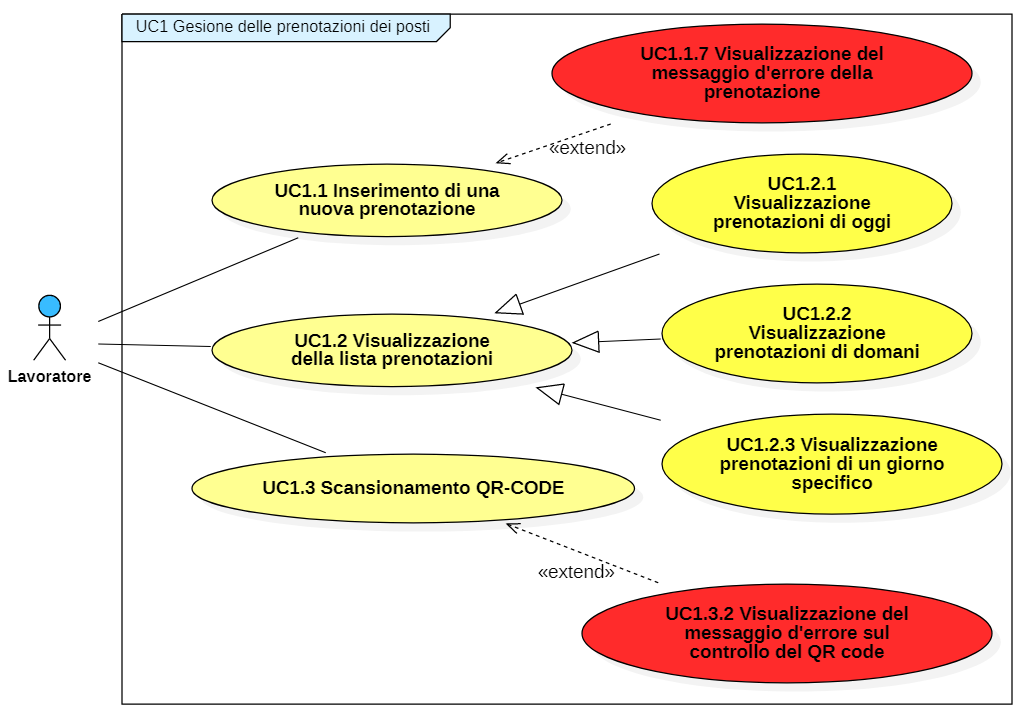
\includegraphics[scale=0.47]{UC1.png}
			\caption{Use Case - UC1:Gestione delle prenotazioni dei posti}\label{fig:UC1}
		\end{center}
	\end{figure}
\usecaseactors{Lavoratore}
\usecasepre{Il lavoratore ha effettuato l'accesso nell'applicazione, è entrato nella sezione Azzurra e ha selezionato la feature UC1 Prenotazione Posto}
\usecasedesc{Il utilizza le funzioni di gestione delle prenotazioni dei posti
	per svolgere una o più delle seguenti azioni:
	\begin{description}
		\item [- UC1.1] Inserimento di una nuova prenotazione;
		\item [- UC1.2] Visualizzazione della lista delle prenotazioni;
		\item [- UC1.3] Scansionamento QR-CODE.
	\end{description}}
\usecasepost{Vengono forniti all'utente i risultati delle funzionalità per la gestione delle prenotazioni.}
\end{usecase}

\begin{usecase}{1.1}{Inserimento di una nuova prenotazione}
	\usecaseactors{Lavoratore}
	\usecasepre{Il lavoratore ha selezionato la funzionalità di prenotazione posto e può inserire un nuova prenotazione di un posto a sedere}
	\usecasedesc{Il lavoratore selezione la funzionalità "Inserisci di una nuova prenotazione".}
	\usecaseflow{
	\begin{description}
		\item Il lavoratore accede alla funzionalità di inserimento di una nuova prenotazione di un posto a sedere;
		\item [- UC1.1.1] Inserisce la data di prenotazione;
		\item [- UC1.1.2] Inserisce l'ora di inizio della prenotazione;
		\item [- UC1.1.3] Inserisce l'ora di terminazione della prenotazione;
		\item [- UC1.1.4] Inserisce la stanza del posto da prenotazione;
		\item [- UC1.1.5] Inserisce il posto da prenotare;
		\item [- UC1.1.6] Visualizza il messaggio di conferma della prenotazione;
\end{description}}
	\usecasealt{Se il tentativo di inserire una nuova prenotazione fallisce viene visualizzato un messaggio d'errore}
	\usecasepost{Il lavoratore ha eseguito il processo d'inserimento di una nuova prenotazione}
	\usecaseest{
		\begin{description}
			\item [- UC1.1.7] Visualizzazione del messaggio d'errore della prenotazione;
		\end{description}
	}
\end{usecase}

\begin{usecase}{1.1.1}{Inserimento data di prenotazione}
	\usecaseactors{Lavoratore}
	\usecasepre{Il lavoratore ha selezionato l'inserimento di una nuova prenotazione}
	\usecasedesc{Il lavoratore inserisce la data desiderata per la prenotazione del posto a sedere.}
	\usecasepost{Il lavoratore ha inserito la data della nuova prenotazione}
\end{usecase}

\begin{usecase}{1.1.2}{Inserimento ora di inizio prenotazione}
	\usecaseactors{Lavoratore}
	\usecasepre{Il lavoratore ha selezionato l'inserimento di una nuova prenotazione}
	\usecasedesc{Il lavoratore inserisce l'ora di inizio desiderata per la prenotazione del posto a sedere.}
	\usecasepost{Il lavoratore ha inserito l'ora di inizio della nuova prenotazione}
\end{usecase}

\begin{usecase}{1.1.3}{Inserimento ora di terminazione prenotazione}
	\usecaseactors{Lavoratore}
	\usecasepre{Il lavoratore ha selezionato l'inserimento di una nuova prenotazione}
	\usecasedesc{Il lavoratore inserisce l'ora di terminazione desiderata per la prenotazione del posto a sedere.}
	\usecasepost{Il lavoratore ha inserito l'ora di terminazione della nuova prenotazione}
\end{usecase}

\begin{usecase}{1.1.4}{Inserimento stanza del posto da prenotare}
	\usecaseactors{Lavoratore}
	\usecasepre{Il lavoratore ha selezionato l'inserimento di una nuova prenotazione}
	\usecasedesc{Il lavoratore inserisce la stanza del posto da prenotare.}
	\usecasepost{Il lavoratore ha inserito la stanza del posto da prenotare}
\end{usecase}

\begin{usecase}{1.1.5}{Inserimento posto da prenotare}
	\usecaseactors{Lavoratore}
	\usecasepre{Il lavoratore ha selezionato l'inserimento di una nuova prenotazione}
	\usecasedesc{Il lavoratore inserisce il posto da prenotare.}
	\usecasepost{Il lavoratore ha inserito il posto da prenotare.}
\end{usecase}

\begin{usecase}{1.1.6}{Visualizzazione del messaggio di conferma della prenotazione}
	\usecaseactors{Lavoratore}
	\usecasepre{Il lavoratore ha inserito i dati della prenotazione}
	\usecasedesc{Il lavoratore ha inserito i dati della prenotazione è riceve il messaggio di conferma della prenotazione.}
	\usecasepost{Il lavoratore riceve il messaggio di conferma della prenotazione.}
\end{usecase}

\begin{usecase}{1.1.7}{Visualizzazione del messaggio d'errore della prenotazione}
	\usecaseactors{Lavoratore}
	\usecasepre{Il lavoratore ha selezionato l'inserimento di una nuova prenotazione}
	\usecasedesc{Con i dati che sono stati inseriti risulta che non ci sono posti liberi, oppure è avvenuto un errore di connessione.}
	\usecasepost{Il lavoratore ha visualizzato il messaggio d'errore}
\end{usecase}

\begin{usecase}{1.2}{Visualizzazione della lista delle prenotazioni}
	\usecaseactors{Lavoratore}
	\usecasepre{Il lavoratore ha selezionato la funzionalità di prenotazione posto e può visualizzare le sue prenotazione}
	\usecasedesc{Il lavoratore vuole visualizzare la lista delle proprie prenotazioni asseconda di una certa modalità.}
	\usecasepost{Il lavoratore ha visualizzato le sue prenotazioni}
	\usecasegen{	
		\begin{description}
			\item [- UC1.2.1] Visualizzazione prenotazioni di oggi;
			\item [- UC1.2.2] Visualizzazione prenotazioni di domani;
			\item [- UC1.2.3] Visualizzazione prenotazioni di un giorno specifico.
		\end{description}}	
\end{usecase}

\begin{usecase}{1.2.1}{Visualizzazione prenotazioni di oggi}
	\usecaseactors{Lavoratore}
	\usecasepre{Il lavoratore ha selezionato la visualizzazione delle sue prenotazioni}
	\usecasedesc{Il lavoratore vuole visualizzare le sue prenotazioni del giorno corrente.}
	\usecasepost{Il lavoratore visualizza le sue prenotazioni del giorno corrente}
\end{usecase}

\begin{usecase}{1.2.2}{Visualizzazione prenotazioni di domani}
	\usecaseactors{Lavoratore}
	\usecasepre{Il lavoratore ha selezionato la visualizzazione delle sue prenotazioni}
	\usecasedesc{Il lavoratore vuole visualizzare le sue prenotazioni di domani.}
	\usecasepost{Il lavoratore visualizza le sue prenotazioni di domani}
\end{usecase}

\begin{usecase}{1.2.3}{Visualizzazione prenotazioni di un giorno specifico}
	\usecaseactors{Lavoratore}
	\usecasepre{Il lavoratore ha selezionato la visualizzazione delle sue prenotazioni}
	\usecasedesc{Il lavoratore vuole visualizzare le sue prenotazioni di uno giorno specifico.}
	\usecasepost{Il lavoratore visualizza le sue prenotazioni di uno giorno specifico}
\end{usecase}

\begin{usecase}{1.3}{Scansionamento  QR-CODE}
	\usecaseactors{Lavoratore}
	\usecasepre{Il lavoratore ha selezionato la funzionalità per scansionamento del QR code per poter riscattare il posto prenotato}
	\usecasedesc{Il lavoratore seleziona la funzionalità "Scansiona QR code" per riscattare il posto prenotato.}
	\usecasealt{Il QR code scansionato è di un posto che non è prenotato dal lavoratore che lo ha scansionato, quindi non può usufruire del posto}
	\usecasepost{Il lavoratore visualizza il messaggio in cui viene comunicato che può utilizza il posto prenotato}
		\usecaseest{
		\begin{description}
			\item [- UC1.3.2] Visualizzazione del messaggio d'errore sul controllo del QR code.
		\end{description}
		}
\end{usecase}

\begin{usecase}{1.3.1}{Visualizzazione messaggio di conferma di riscatto del posto prenotato}
	\usecaseactors{Lavoratore}
	\usecasepre{Il lavoratore ha scansionato il QR code del posto prenotato}
	\usecasedesc{Lo scansionato del QR code del posto prenotato e il successivo controllo, ha dato esito positivo.}
	\usecasepost{Il lavoratore visualizza il messaggio di conferma}
\end{usecase}

\begin{usecase}{1.3.2}{Visualizzazione del messaggio d'errore sul controllo del QR code}
	\usecaseactors{Lavoratore}
	\usecasepre{Il lavoratore ha scansionato il QR code del posto prenotato}
	\usecasedesc{Lo scansionato del QR code del posto prenotato e il successivo controllo, ha dato esito negativo perché c'è stato un errore o perché il posto non è riservato a chi ha scansionato il QR code.}
	\usecasepost{Il lavoratore visualizza il messaggio d'errore}
\end{usecase}

\section{Gestione delle prenotazioni dei posti}
